\documentclass[10pt]{beamer}
\usepackage{etex}
\usetheme[
%%% options passed to the outer theme
%    progressstyle=fixedCircCnt,   %either fixedCircCnt, movCircCnt, or corner
%    rotationcw,          % change the rotation direction from counter-clockwise to clockwise
%    shownavsym          % show the navigation symbols
  ]{AAUsimple}

% If you want to change the colors of the various elements in the theme, edit and uncomment the following lines
% Change the bar and sidebar colors:
%\setbeamercolor{AAUsimple}{fg=green!20,bg=green}
%\setbeamercolor{sidebar}{bg=red!20}
% Change the color of the structural elements:
%\setbeamercolor{structure}{fg=red}
% Change the frame title text color:
%\setbeamercolor{frametitle}{fg=blue}
% Change the normal text color background:
%\setbeamercolor{normal text}{fg=black,bg=gray!10}
% ... and you can of course change a lot more - see the beamer user manual.

\usepackage[utf8]{inputenc}
\usepackage[english]{babel}
\usepackage[T1]{fontenc}
% Or whatever. Note that the encoding and the font should match. If T1
% does not look nice, try deleting the line with the fontenc.
\usepackage{helvet}
\usepackage{xcolor}

%use for graphics
\usepackage{calc}
\usepackage{ifthen}
\usepackage{amsmath,amsfonts,amssymb,amsthm}
\usepackage{mathtools}
\usepackage{todonotes}

% Todo commands

\newcommand{\todoin}[2][]{\todo[inline, color=blue!40, #1]{#2}}
\newcommand{\fixme}[2][]{\todo[color=yellow!40, #1]{#2}}
\newcommand{\fixmein}[2][]{\todo[inline, color=yellow!40, #1]{#2}}


\usepackage{tikz}
\usetikzlibrary{arrows, automata, positioning}
\DeclarePairedDelimiter{\ceil}{\lceil}{\rceil}
\DeclarePairedDelimiter{\floor}{\lfloor}{\rfloor}
\DeclarePairedDelimiter{\tuple}{\langle}{\rangle}
\newcommand{\darrow}{\, \downarrow \!\!}
\newcommand{\uarrow}{\, \uparrow \!\!}

%other package for graphics

%\usepackage{pstricks}
%\usepackage{pstricks-add}

%\usepackage{pst-plot}
\usepackage{xcolor,colortbl}

\newcommand{\mc}[2]{\multicolumn{#1}{c}{#2}}
\definecolor{Gray}{gray}{0.85}

\newcolumntype{a}{>{\columncolor{Gray}}c}
\newcolumntype{b}{>{\columncolor{white}}c}

% command for slices graphic
\newcommand{\slice}[4]{
  \pgfmathparse{0.5*#1+0.5*#2}
  \let\midangle\pgfmathresult

  % slice
  \draw[thick,fill=black!10] (0,0) -- (#1:1) arc (#1:#2:1) -- cycle;

  % outer label
  \node[label=\midangle:#4] at (\midangle:1) {};

  % inner label
  \pgfmathparse{min((#2-#1-10)/110*(-0.3),0)}
  \let\temp\pgfmathresult
  \pgfmathparse{max(\temp,-0.5) + 0.8}
  \let\innerpos\pgfmathresult
  \node at (\midangle:\innerpos) {#3};
}
% colored hyperlinks
\newcommand{\chref}[2]{%
  \href{#1}{{\usebeamercolor[bg]{AAUsimple}#2}}%
}


\title{ACS and MMAS \\ for the Permutation Flow Shop Problem \\ with Weighted Tardiness}
\subtitle{Swarm Intelligence project}

\date{June 17, 2019}

\author{
  Hakim \textsc{Boulahya}
}

% - Give the names in the same order as they appear in the paper.
% - Use the \inst{?} command only if the authors have different
%   affiliation. See the beamer manual for an example

\institute[
%  {\includegraphics[scale=0.2]{aau_segl}}\\ %insert a company, department or university logo
  Faculty of Science
  Université Libre de Bruxelles
  Belgium
] % optional - is placed in the bottom of the sidebar on every slide
{% is placed on the bottom of the title page

  Département d'Informatique \\
  Université Libre de Bruxelles \\
  %there must be an empty line above this line - otherwise some unwanted space is added between the university and the country (I do not know why;( )
}

% specify a logo on the titlepage (you can specify additional logos an include them in
% institute command below
\pgfdeclareimage[height=1.5cm]{titlepagelogo}{img/logoULB} % placed on the title page
\titlegraphic{% is placed on the bottom of the title page
  \pgfuseimage{titlepagelogo}
%  \hspace{1cm}\pgfuseimage{titlepagelogo2}
}
\definecolor{firstcolor}{RGB}{0, 76, 146}
\definecolor{secondcolor}{RGB}{43,46,62}
\definecolor{thirdcolor}{RGB}{180,200,212}

\begin{document}
% the titlepage
{\aauwavesbg%
\begin{frame}[plain,noframenumbering] % the plain option removes the header from the title page
  \titlepage
\end{frame}}
%%%%%%%%%%%%%%%%
%%%%%%%%%%%%%%%%

% TOC
\begin{frame}{Contents}{}

%\centering \textit{\large The involvment of Facebook in the learning process}
\begin{block}{}
  \textbf{Project}: ACO Algorithms for PFSP-WT
  \begin{enumerate}
    \item \textcolor{firstcolor}{\textbf{Algorithms and implementation}}
    \item \textcolor{firstcolor}{\textbf{Adding local search routine}}
     \item \textcolor{firstcolor}{\textbf{Results and comparisons}}
    \item \textcolor{firstcolor}{\textbf{Conclusion}}
  \end{enumerate}
\end{block}

\end{frame}

\section{Algorithms}

\begin{frame}{Implementation}{}
    \begin{itemize}
      \item Schedule construction by exploiting with probability $q_0$:
      \begin{itemize}
        \item Exploit. best schedule: $\mathrm{argmax}_{unscheduled}(\tau_{ij})^\alpha (\eta_{ij})^\beta$
        \item Biased exploration: $p_{ij} = \frac{(\tau_{ij})^\alpha (\eta_{ij})^\beta}{\sum_{unscheduled}{(\tau_{ij})^\alpha (\eta_{ij})^\beta}}$
      \end{itemize}
      \item Earliest Due Dates (EDD) heursitic for initialization: Sort by due dates and $\eta_{ij} = 1 / d_i$
      \item Global pheromone update applied only by best-iteration ant (using $\rho$ for evaporation)
    \end{itemize}
    \begin{columns}[T]
     \begin{column}{.5\textwidth}
         \begin{block}{ACS}
            \begin{itemize}
              \item Include local pheromone update during ant's solution build (using $\xi$)
              \item $\tau_0$ based on EDD solution
            \end{itemize}
         \end{block}
       \end{column}
       \begin{column}{.5\textwidth}
           \begin{block}{MMAS}
               \begin{itemize}
                   \item $q_0 = 0$: only explore
                   \item Pheromone interval: $\tau_{min} \le \tau_{ij} \le \tau_{max}$
                   \item Interval updated at each iteration based on current best solution
               \end{itemize}
           \end{block}
       \end{column}
   \end{columns}
\end{frame}


\section{Local search}

\begin{frame}{Local search}{}

Local search performed using exhaustive \textit{insertion-moves}:

\begin{itemize}
  \item That is for all permutation $(i, j)$, remove job from position $i$ and insert it in position $j$
  \item Performs in $O(n^2)$ for a schedule
\end{itemize}


% \\~\\~\\

Two mechanisms implemented:

\begin{itemize}
  \item \textit{best-ant}: Only best-iteration ant can perform local search: $O(n^2)$ per iteration
  \item \textit{all-ant}: All ant can perform local search: $O(mn^2)$ per iteration
\end{itemize}

\end{frame}

\section{Results}

\begin{frame}{Results}{Setup}

\begin{itemize}
  \item Because local search routine appears to have a big impact on solution quality, we compare the results of the following 6 algorithms:
  \begin{itemize}
    \item ACS
    \item MMAS
    \item ACS-LS-BEST (ALB)
    \item ACS-LS-ALL (ALA)
    \item MMAS-LS-BEST (MLB)
    \item MMAS-LS-ALL (MLA)
  \end{itemize}
  \item Execution of each algorithm on each instance 10 times
  \item One execution = 30 seconds time budget
\end{itemize}

\end{frame}

\begin{frame}{Results}{Parameters}

\textbf{Best configurations parameters returned by \texttt{irace} for each algorithm}


% \begin{table}[]
\begin{center}

\begin{tabular}{ | l | c | c | c | c | c | c | c | }
  \hline
      & ACS    & MMAS    & ALB & ALA & MLB & MLA \\
  \hline
  ants         & 41     & 28      & 5        &  93   & 34  & 87 \\
  \hline
  $\alpha$     & 2.56   & 3.88    & 2.83     &  3.69    &   4.41     & 0.34 \\
  \hline
  $\beta$      & 7.78   & 6.69    & 3.28     &  5.08     & 9.48      & 6.76 \\
  \hline
  $\rho$       & 0.32   & 0.53    & 0.61     &  0.05      &   0.41     & 0.7 \\
  \hline
  $\xi$        & 0.46   & -       & 0.38     &  0.77     &       -      & - \\
  \hline
  $q_0$        & 0.07   & -       & 0.04     &  0.24    &       -      & - \\
  \hline

\end{tabular}
% \caption{Parameters tuned and best configurations returned by \texttt{irace} for each algorithm}
% \label{table:irace}
% \end{table}
\end{center}

% \\~\\

Observations:
\begin{itemize}
  \item When \textit{all-ant} is used, \texttt{irace}  returns nearly max. of ants
  \item $q_0$ mostly very low, exploration seems to perform better
  \item Heuristic desirability has bigger impact than pheromone trails
  % \item Pheromones evaporation ??
\end{itemize}

\end{frame}


\begin{frame}{Results}{Boxplot}
    \begin{columns}[T]
     \begin{column}{.5\textwidth}
         \begin{block}{Instance with 50 jobs}
         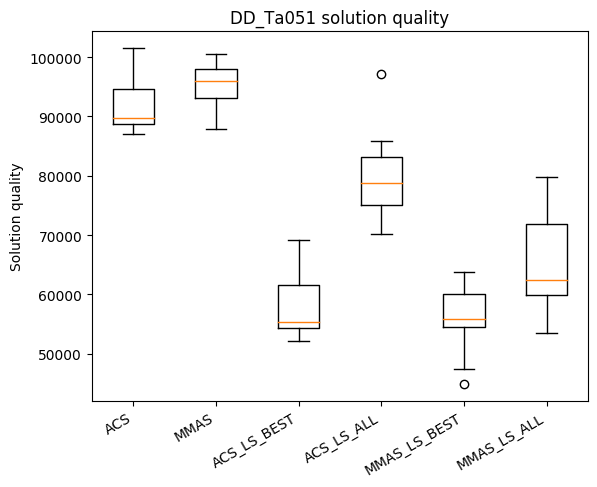
\includegraphics[scale=0.3]{plots/DD_Ta051__boxplot}
         \end{block}
       \end{column}
       \begin{column}{.5\textwidth}
         \begin{block}{Instance with 100 jobs}
         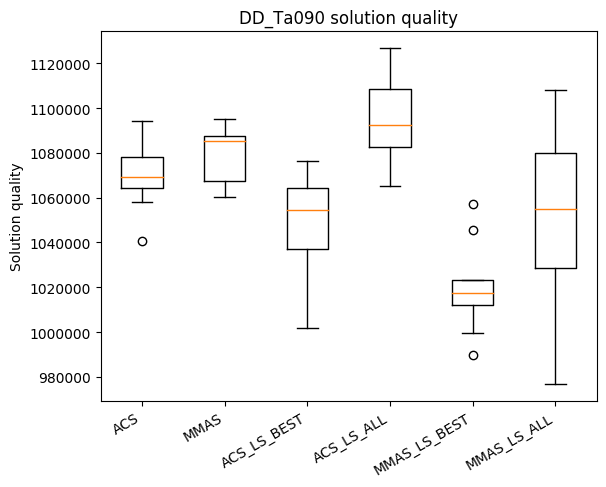
\includegraphics[scale=0.3]{plots/DD_Ta090__boxplot}
         \end{block}
       \end{column}
   \end{columns}
\end{frame}


\begin{frame}{Results}{Convergence}
    \begin{columns}[T]
     \begin{column}{.5\textwidth}
         \begin{block}{Instance with 50 jobs}
         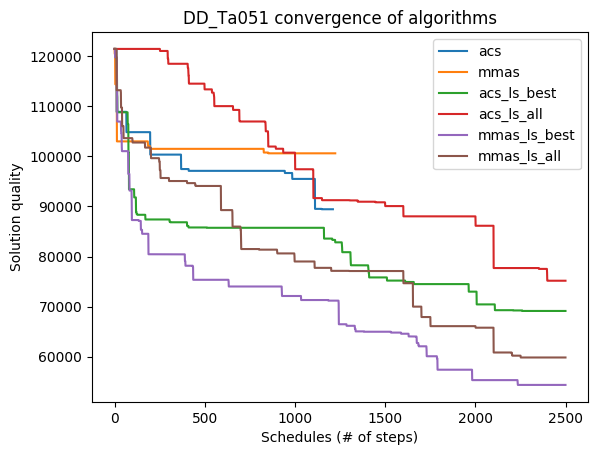
\includegraphics[scale=0.3]{plots/DD_Ta051__best_runs_convergence}
         \end{block}
       \end{column}
       \begin{column}{.5\textwidth}
         \begin{block}{Instance with 100 jobs}
         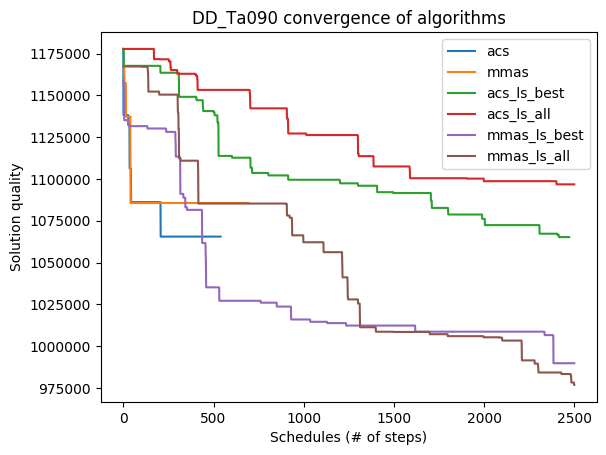
\includegraphics[scale=0.3]{plots/DD_Ta090__best_runs_convergence}
         \end{block}
       \end{column}
   \end{columns}
\end{frame}

\begin{frame}{Results}{Best total weighted tardiness}

\begin{itemize}
  \item Best results repartition for all 20 instances
  \begin{itemize}
    \item ACS: 0\%
    \item MMAS: 0\%
    \item ACS-LS-BEST: 40\%
    \item ACS-LS-ALL: 0\%
    \item MMAS-LS-BEST: 35\%
    \item MMAS-LS-ALL: 25\%
  \end{itemize}
\end{itemize}

\end{frame}

\begin{frame}{Conclusion}{}
\begin{itemize}
  \item Intuitive observations
  \begin{itemize}
    \item \textit{best-ant} local search seems to always performs better
    \item MMAS-LS-BEST seems better for instances with fewer jobs and ACS-LS-BEST for instances with more jobs
  \end{itemize}
  \item Improvements
  \begin{itemize}
    \item No parameters analysis..
    \item No analysis of MMAS stagnation and parameters reinitialization
  \end{itemize}
\end{itemize}
\end{frame}



%%%%%%%%%%%%%%%%

{\aauwavesbg
% \begin{frame}[allowframebreaks]
    % \frametitle{References}
% \bibliographystyle{plain}
% \bibliography{../thesis}
% \end{frame}}

{\aauwavesbg
\begin{frame}[plain,noframenumbering]
  \finalpage{Thank you!}
\end{frame}}

\end{document}
